\documentclass[a4paper,14pt]{extarticle}

\usepackage[utf8x]{inputenc}
\usepackage[T1,T2A]{fontenc}
\usepackage[russian]{babel}
\usepackage{hyperref}
\usepackage{indentfirst}
\usepackage{here}
\usepackage{array}
\usepackage{graphicx}
\usepackage{caption}
\usepackage{subcaption}
\usepackage{chngcntr}
\usepackage{amsmath}
\usepackage{amssymb}
\usepackage{pgfplots}
\usepackage{pgfplotstable}
\usepackage[left=2cm,right=2cm,top=2cm,bottom=2cm,bindingoffset=0cm]{geometry}
\usepackage{multicol}

\renewcommand{\le}{\ensuremath{\leqslant}}
\renewcommand{\leq}{\ensuremath{\leqslant}}
\renewcommand{\ge}{\ensuremath{\geqslant}}
\renewcommand{\geq}{\ensuremath{\geqslant}}
\renewcommand{\epsilon}{\ensuremath{\varepsilon}}
\renewcommand{\phi}{\ensuremath{\varphi}}

\counterwithin{figure}{section}
\counterwithin{equation}{section}
\counterwithin{table}{section}
\newcommand{\sign}[1][5cm]{\makebox[#1]{\hrulefill}} % Поля подписи и даты
\graphicspath{{pics/}} % Путь до папки с картинками
\captionsetup{justification=centering,margin=1cm}
\def\arraystretch{1.3}

\begin{document}

\begin{titlepage}
\begin{center}
	\textbf{Санкт-Петербургский Политехнический Университет \\Петра Великого}\\[0.3cm]
	\small Институт компьютерных наук и технологий \\[0.3cm]
	\small Кафедра компьютерных систем и программных технологий\\[4cm]
	
	\textbf{ОТЧЕТ}\\ \textbf{о лабораторной работе}\\[0.5cm]
	\textbf{<<Исследование частотных характеристик пассивных RC-цепей>>}\\[0.1cm]
	\textbf{Электротехника и Электроника}\\[10.5cm]
\end{center}

\begin{flushright}
	\begin{minipage}{0.60\textwidth}
		\begin{flushleft}
			\small \textbf{Работу выполнили студенты}\\[3mm]
			\small группа 23501/4 \hspace*{17mm} Дьячков В.В.\\[3mm]
			\small группа 23501/4 \hspace*{17mm} Ламтев А.Ю.\\[5mm]
			
			\small \textbf{Преподаватель}\\[5mm]
		 	\small \sign[3.5cm] \hspace*{8mm} к.т.н., доц. Кочетков Ю.Д.\\[0.5cm]
		\end{flushleft}
	\end{minipage}
\end{flushright}

\vfill

\begin{center}
	\small Санкт-Петербург\\
	\small \the\year
\end{center}
\end{titlepage}

\section{Цель работы}

Приобретение навыков настройки и исследования импульсных генераторов (автоколебательных и ждущих), определения областей применения различных интегральных микросхем в генераторах.

\section{Чертеж схемы исследуемого устройства}

\begin{figure}[H]
\begin{center}
	\begin{subfigure}[b]{0.35\textwidth}
		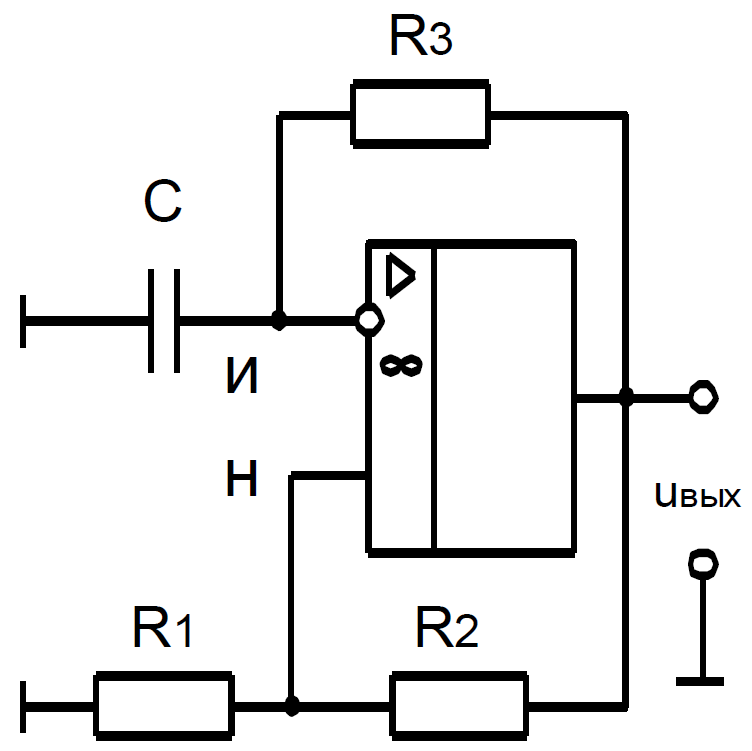
\includegraphics[scale=0.3]{scheme1}
		\caption{Симметричный мультивибратор}
	\end{subfigure}
	~
	\begin{subfigure}[b]{0.35\textwidth}
		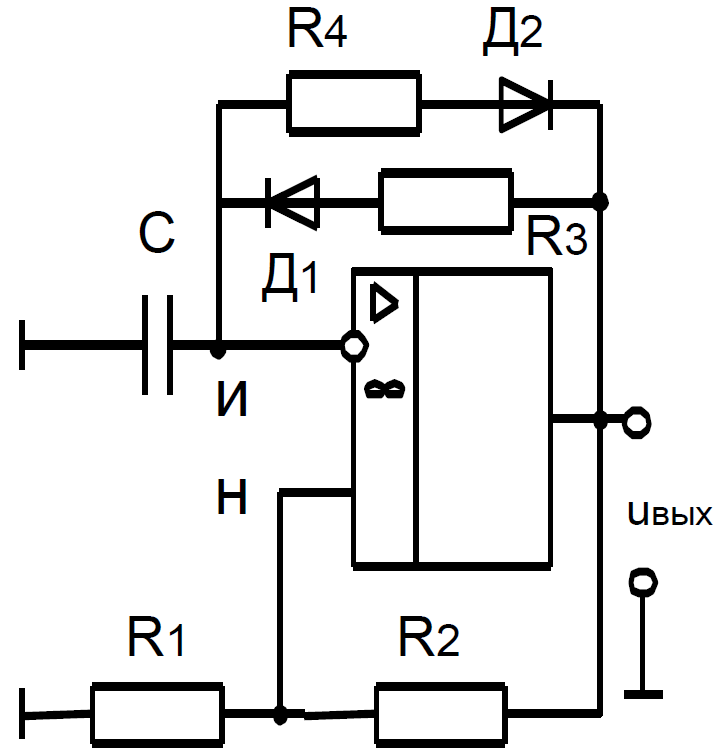
\includegraphics[scale=0.3]{scheme2}
		\caption{Несимметричный мультивибратор}
	\end{subfigure}
	~
	\begin{subfigure}[b]{0.35\textwidth}
		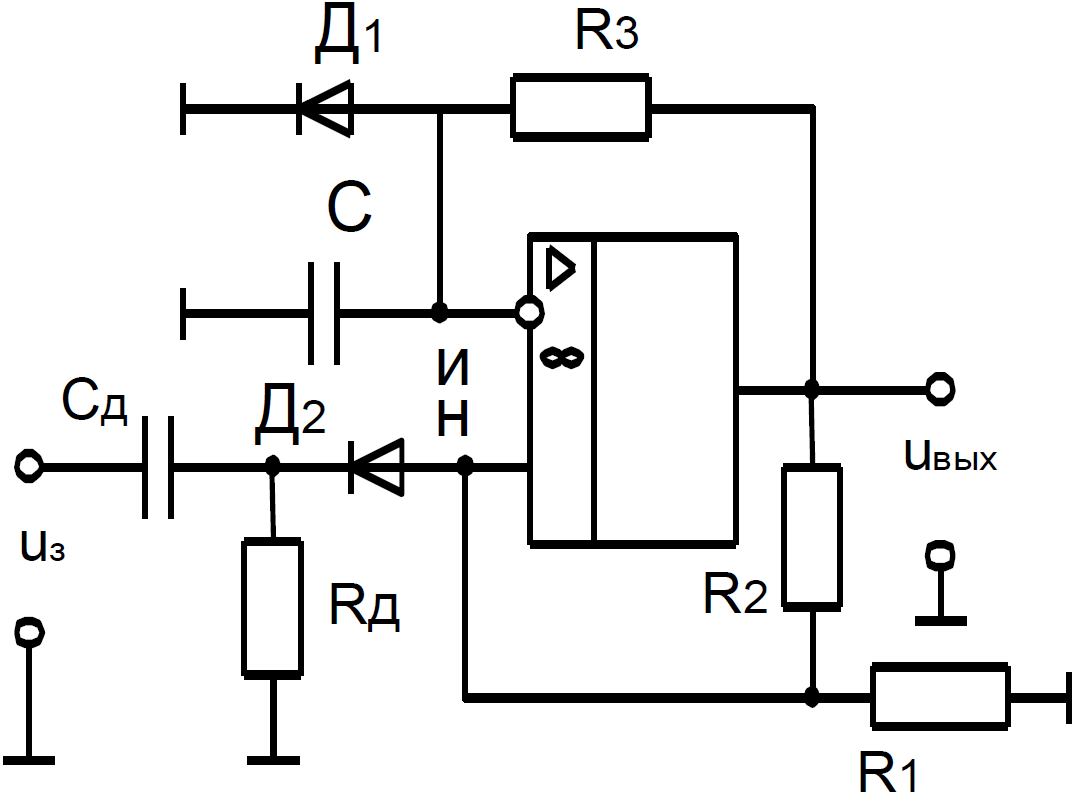
\includegraphics[scale=0.3]{scheme3}
		\caption{Ждущий генератор}
	\end{subfigure}
	\caption{}
\end{center}
\end{figure}


\section{Исходные данные}

Операционный усилитель \verb+К140УД6+.

\begin{table}[H]
\begin{center}
	\caption{Исходные данные}
	\def\tabcolsep{10pt}
	\begin{tabular}{|c|c|c|c|c|c|c|c|}
		\hline
		$t_{\text{и1}}$, мкс &
		$t_{\text{и2}}$, мкс &
		$K_{\text{Д}}$ &
		$C$, нФ &
		$R_{\text{Д}}$, кОм &
		$C_{\text{Д}}$, пФ &
		$E_{01}$, В &
		$E_{02}$, В \\
		\hline
		20 &
		40 &
		1 &
		3 &
		10 &
		1500 &
		15 &
		-15 \\
	    \hline	
	\end{tabular}
\end{center}
\end{table}

\section{Теоретические расчёты}

\subsection{Расчёт параметров элементов}

$K_\text{Д} = 1 \Rightarrow$ $R_1 = R_2$. Пусть $R_1 = 20$ кОм, тогда $R_2 = 20$ кОм

\begin{displaymath}
	R_3 = \frac{t_{\text{и1}}}{C \cdot ln(1 + \frac{2R_1}{R_2})} = \frac{20 \cdot 10^{-6}}{3 \cdot 10^9 \cdot ln(1 + 2)} = 6 \text{ кОм}
\end{displaymath}

\begin{displaymath}
	R_4 = \frac{t_{\text{и2}}}{C \cdot ln(1 + \frac{2R_1}{R_2})} = \frac{40 \cdot 10^{-6}}{3 \cdot 10^9 \cdot ln(1 + 2)} = 12 \text{ кОм}
\end{displaymath} 

\subsection{Расчёт $t_\text{имп}$ симметричного мультивибратора}

\begin{equation}
	\label{eq:4:1}
	t_{\text{и1}} = R_3 C ln\left(1 + \frac{\left(1 - \frac{U_\text{вых}^{-}}{U_\text{вых}^{+}}\right) R_1}{R_2}\right) 
\end{equation}

\begin{displaymath}
	t_{\text{и1}} = 6 \cdot 10^3 \cdot 3 \cdot 10^{-9} \cdot ln\left(1 + \frac{\left(1 - \frac{-15}{0.7 \cdot 15}\right)\cdot 20 \cdot 10^3}{20 \cdot 10^3}\right) = 22.2 \text{ мкс}
\end{displaymath}

\begin{equation}
	\label{eq:4:2}
	t_{\text{и2}} = R_3 C ln\left(1 + \frac{\left(1 - \frac{U_\text{вых}^{+}}{U_\text{вых}^{-}}\right) R_1}{R_2}\right) 
\end{equation}

\begin{displaymath}
	t_{\text{и2}} = 6 \cdot 10^3 \cdot 3 \cdot 10^{-9} \cdot ln\left(1 + \frac{\left(1 - \frac{0.7 \cdot 15}{-15}\right)\cdot 20 \cdot 10^3}{20 \cdot 10^3}\right) = 17.9 \text{ мкс}
\end{displaymath}

\begin{displaymath}
	t_{\text{и}} = \frac{t_{\text{и1}} + t_{\text{и2}}}{2} = \frac{22.2 + 17.9}{2} = 20.1 \text{ мкс}
\end{displaymath}

\subsection{Расчёт $t_\text{имп}$ несимметричного мультивибратора}

\begin{equation}
	\label{eq:4:3}
	t_{\text{и1}} = R_3 C ln\left(1 + 2 \cdot \frac{R_1}{R_2}\right) 
\end{equation}

\begin{displaymath}
	t_{\text{и1}} = 6 \cdot 10^3 \cdot 3 \cdot 10^{-9} \cdot ln\left(1 + 2 \cdot \frac{20 \cdot 10^3}{20 \cdot 10^3} \right) = 19.8 \text{ мкс}
\end{displaymath}

\begin{equation}
	\label{eq:4:4}
	t_{\text{и2}} = R_4 C ln\left(1 + 2 \cdot \frac{R_1}{R_2}\right) 
\end{equation}

\begin{displaymath}
	t_{\text{и2}} = 12 \cdot 10^3 \cdot 3 \cdot 10^{-9} \cdot ln\left(1 + 2 \cdot \frac{20 \cdot 10^3}{20 \cdot 10^3} \right) = 39.6 \text{ мкс}
\end{displaymath}

\subsection{Расчёт $t_\text{имп}$ ждущего генератора}

\begin{equation}
	\label{eq:4:5}
	t_{\text{и}} = R_3 C ln\left(1 + \frac{R_1}{R_2}\right) 
\end{equation}

\begin{displaymath}
	t_{\text{и}} = 6 \cdot 10^3 \cdot 3 \cdot 10^{-9} \cdot ln\left(1 + \frac{20 \cdot 10^3}{20 \cdot 10^3}\right) = 12.5 \text{ мкс} 
\end{displaymath}

\begin{equation}
	\label{eq:4:6}
	t_{\text{в}} = R_3 C ln\left(1 + \frac{\frac{R_1}{R_2}}{1 + \frac{R_1}{R_2}}\right)
\end{equation}

\begin{displaymath}
	t_{\text{в}} = 6 \cdot 10^3 \cdot 3 \cdot 10^{-9} \cdot ln\left(1 + \frac{\frac{20 \cdot 10^3}{20 \cdot 10^3}}{1 + \frac{20 \cdot 10^3}{20 \cdot 10^3}}\right) = 7.30 \text{ мкс}
\end{displaymath}

\newpage

\section{Экспериментально снятые зависимости}

\subsection{Симметричный мультивибратор}

При $R_3 = 6$ кОм: $t_\text{и} = 22$ мкс.

\begin{figure}[H]
\begin{center}
	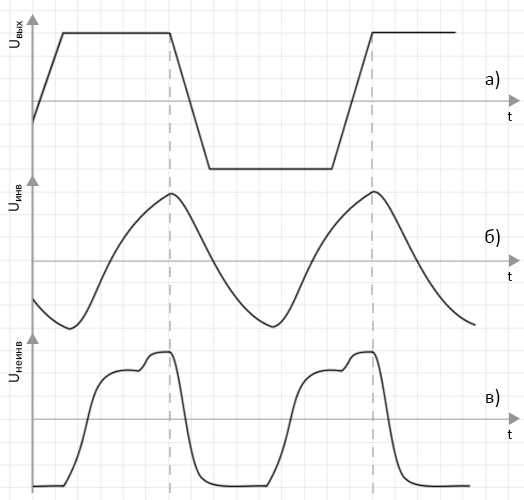
\includegraphics[width=0.81\textwidth]{first_scheme}
	\captionsetup{margin=0cm}
	\caption{Временная диаграмма симметричного мультивибратора:\\ а) $U_\text{вых}$, б) $U_\text{инв}$, в) $U_\text{неинв}$.} 
	\label{fig:diff}
\end{center}
\end{figure}

Установив $E_{01} = 0.7 E_\text{0\ ном}$, получили $t_\text{и} = 22.25$ мкс.

\subsection{Несимметричный мультивибратор}

Взяв $R_3 = 6$ кОм и $R_4 = 12$ кОм, получили:

\begin{table}[H]
\begin{center}
	\caption{Результаты измерений}
	\def\tabcolsep{10pt}
	\begin{tabular}{|c|c|}
		\hline
		$t_{\text{и1}}$, мкс &
		$t_{\text{и2}}$, мкс \\
		\hline
		23.5 &
		33.8 \\
	    \hline	
	\end{tabular}
\end{center}
\end{table}

Затем последовательно уменьшая $R_4$, получили $R_4 = 560$ Ом, при котором $t_{\text{и2}} = 7$ мкс и достигается максимальное значение частоты работы мультивибратора на данном типе ОУ $f_{max} = 71.43$ кГц.

\subsection{Ждущий генератор}

Взяв $R_3 = 6$ кОм, $R_4 = 12$ кОм, $R_\text{Д} = 10$ кОм и $C_\text{Д} = 1.5$ нФ, получили:

\begin{figure}[H]
\begin{center}
	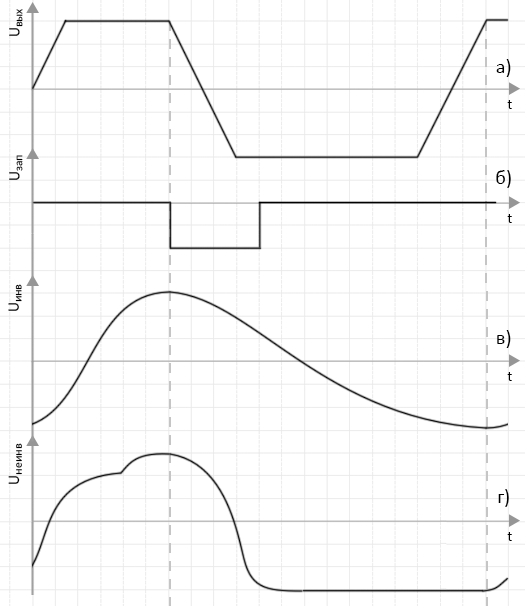
\includegraphics[width=0.81\textwidth]{whynot}
	\captionsetup{margin=0cm}
	\caption{Временная диаграмма ждущего генератора:\\ а) $U_\text{вых}$, б) $U_\text{зап}$, в) $U_\text{инв}$, г) $U_\text{неинв}$.} 
	\label{fig:diff}
\end{center}
\end{figure}

\begin{table}[H]
\begin{center}
	\caption{Результаты измерений}
	\def\tabcolsep{10pt}
	\begin{tabular}{|c|c|c|}
		\hline
		$U_\text{зап\ min}$, В &
		$t_\text{зап\ min}$, мкс &
		$t_{\text{восст}}$, мкс \\
		\hline
		3.8 &
		9 &
		6.7 \\
	    \hline	
	\end{tabular}
\end{center}
\end{table}

\begin{table}[H]
\begin{center}
	\caption{Зависимость длительности импульса $t_\text{имп}$ от емкости конденсатора $C$.}
	\label{tab:limiter}
	\def\tabcolsep{20pt}
	\def\arraystretch{1.23}
	\fontsize{13}{14}\selectfont
	\pgfplotstabletypeset[col sep=comma,
	    columns={c,t},
	    column type/.add={|c|}{},
	    columns/c/.style={fixed, column name={$t_\text{имп}$, мкс}},
	    columns/t/.style={fixed, column name={$C$, нФ}},
	    every nth row={1}{before row=\hline},
	    every head row/.style={before row=\hline, after row=\hline},
	    every last row/.style={after row=\hline}
	   ]{data/c.csv}
\end{center}
\end{table}

\vspace{-1cm}

\begin{figure}[H]
\begin{center}
	\begin{tikzpicture} [every plot/.append style={thick}]
		\begin{axis}[
			x tick label style={
				/pgf/number format/.cd,
				fixed,
				precision=2,
				/tikz/.cd
			},
			height=0.3\textheight,
			width=0.75\textwidth,
			legend pos = north east,
			xlabel={$C$, нФ},
			ylabel={$t_\text{имп}$, мкс},
			axis x line = middle,
			axis y line = middle,
			xmax = 550,
			ymax = 1400,
			grid=major
		]
		\addplot table[x=c,y=t,col sep=comma]{data/c.csv};
		\end{axis}
	\end{tikzpicture}
	\caption{Зависимость длительности импульса $t_\text{имп}$ от емкости конденсатора $C$.}
	\label{plot:limiter_detail}
\end{center}
\end{figure}

\newpage

\section{Погрешности}

\subsection{Предельно допустимая погрешность}

\begin{displaymath}
\begin{aligned}
		\delta_{max} t_{\text{и}} = \delta_{max} t_{\text{в}} =\sqrt{\sqrt{\delta R_1} + \sqrt{\delta R_2} + (\delta R_3)^2 + (\delta C)^2} = \\ = \sqrt{\sqrt{0.1} + \sqrt{0.1} + 0.1^2 + 0.1^2} = 0.807 = 80.7 \%
\end{aligned}
\end{displaymath}

\subsection{Симметричный мультивибратор}

\begin{displaymath}
	\delta t_{\text{и}} = \left| \frac{t_{\text{и теор}} - t_{\text{и эксп}}}{t_{\text{и теор}}} \right| = \left| \frac{20.1 - 22}{20.1} \right| = 0.0945 = 9.45 \% < \delta_{max} t_{\text{и}} = 80.7 \%
\end{displaymath}

\subsection{Несимметричный мультивибратор}

\begin{displaymath}
	\delta t_{\text{и1}} = \left| \frac{t_{\text{и1 теор}} - t_{\text{и1 эксп}}}{t_{\text{и1 теор}}} \right| = \left| \frac{19.8 - 23.5}{19.8} \right| = 0.187 = 18.7 \% < \delta_{max} t_{\text{и}} = 80.7 \%
\end{displaymath}

\begin{displaymath}
	\delta t_{\text{и2}} = \left| \frac{t_{\text{и2 теор}} - t_{\text{и2 эксп}}}{t_{\text{и2 теор}}} \right| = \left| \frac{39.6 - 38.8}{39.6} \right| = 0.0202 = 2.02 \% < \delta_{max} t_{\text{и}} = 80.7 \%
\end{displaymath}

\subsection{Ждущий генератор}

\begin{displaymath}
	\delta t_{\text{и}} = \left| \frac{t_{\text{и теор}} - t_{\text{и эксп}}}{t_{\text{и теор}}} \right| = \left| \frac{12.5 - 10.2}{12.5} \right| = 0.184 = 18.4 \% < \delta_{max} t_{\text{и}} = 80.7 \%
\end{displaymath}

\begin{displaymath}
	\delta t_{\text{в}} = \left| \frac{t_{\text{в теор}} - t_{\text{в эксп}}}{t_{\text{в теор}}} \right| = \left| \frac{7.30 - 6.7}{7.30} \right| = 0.0821 = 8.21 \% < \delta_{max} t_{\text{в}} = 80.7 \%
\end{displaymath}

\section{Выводы}

Приведённые погрешности полученных в ходе эксперимента значений $t_{\text{и}}$, $t_{\text{и1}}$, $t_{\text{и2}}$ и $t_{\text{в}}$ не превышают предельно допустимые погрешности.

Таким образом, формулы \ref{eq:4:1} -- \ref{eq:4:6} являются верными.

\end{document}